\documentclass[11pt]{article} 
\usepackage{geometry}
\geometry{letterpaper}

\usepackage{graphicx}   
\usepackage{amssymb}
\usepackage{tabularx}
\usepackage{float}
\usepackage{./framed}
\usepackage{hyperref}
\hypersetup{
    colorlinks,
    citecolor=black,
    filecolor=black,
    linkcolor=black,
    urlcolor=blue
}

\usepackage[english]{babel}

\begin{document}

\begin{titlepage}
	\newcommand{\HRule}{\rule{\linewidth}{0.2mm}}
	\begin{center}
	\textsc{\LARGE McMaster University}\\[1.5cm]
	
	\textsc{\Large HydroSwarm}\\[0.5cm]
	\textsc{\large Software \& Mechatronics Capstone}\\[0.5cm] 

	\HRule\\[0.4cm]
		{\huge\bfseries Development Process \& Implementation}\\[0.4cm]
	\HRule\\[0.4cm]
	
	\begin{minipage}[t][][t]{0.5\textwidth}
		\begin{flushleft} \large
			\emph{Authors:}\\
			Victor Velechovsky - \textit{001305263}\\
			Gabriel Potter - \textit{001429884}\\
			Amandeep Panesar - \textit{001431191} \\
			Taha Mian  - \textit{001417172}\\
			Nishanth Balamohan - \textit{001411319} \\
		\end{flushleft}
	\end{minipage}
	~
	\begin{minipage}[t][][t]{0.4\textwidth}
		\begin{flushright} \large
			\emph{Professor:} \\
			Dr. Alan Wassyng \\[0.4cm]
		\end{flushright}
	\end{minipage}\\[2cm]
	
	
\includegraphics[width=0.3\textwidth]{logo.png} \\
	{\large Last compiled on \today}
	\end{center}

\end{titlepage}

\tableofcontents
\listoffigures

\vfill
\begin{figure}[htbp]
   \centering
   \noindent\begin{tabularx}{\textwidth}{| >{\centering\arraybackslash}m{0.2\textwidth} | >{\centering\arraybackslash}m{0.2\textwidth} | >{\centering\arraybackslash}m{0.2\textwidth} | >{\centering\arraybackslash}m{0.285\textwidth} |}
   \hline 
   \textbf{Date} & \textbf{Revision} & \textbf{Comments} & \textbf{Author(s)} \\
   \hline
   Nov. 29 & 1.0 & Template added & Amandeep Panesar \\ \hline
   Nov. 29 & 1.1 & Added sections: Introduction, Team Members, Version Control, Workflow & All authors \\ \hline
   Nov. 30 & 1.2 & Final revision & All authors \\ \hline
   \end{tabularx}
   \caption{Revision History}
\end{figure}

\newpage

\section{Introduction}
\subsection{Project Overview}

HydroSwarm is a swarm of autonomous robotic boats meant to carry out measurements over large bodies of water. For our project, these boats will be measuring water temperature, but the idea can be expanded to any number of other quantifiable measurements. Central to our work will be two major components. First, a small motorized boat, attached with a water temperature sensor, as well as a control unit that allows it to communicate with – and be controlled by – a centralized control unit. Second, a software package that can control a large group (\hyperref[sec:definitions]{swarm}) of these boats, with an algorithm focused on producing reliable, accurate, and fast measurements.\\

Our swarm will aim to cover large areas more quickly and cost-effectively than traditional products. To test the applicability of our project, we will demo it on a small scale body of water, such as a swimming pool, as well as develop a simulation to hypothetically prove the efficacy of the system on a larger scale.\\

Our project will be conducted between Fall 2018 –- Winter 2019 for our Engineering Capstone project at McMaster University, under the guidance of Dr. Alan Wassyng. We have four Software Engineering students, and one Mechatronics Engineering student.

\subsection{Naming Conventions and Terminology}

\label{sec:definitions}
\begin{itemize}
\item \textbf{System}: The entire software and hardware package - including the boats,
boat hardware, control software, and server running the control software
\item \textbf{Swarm}: A large group of objects (in our case, motorized boats) that can communicate and perform acts as a group
\item \textbf{Insect}: A member of the swarm (in our case, a single motorized boat)
\item \textbf{Simulation}: The simulation will be used for demo purposes, mainly to show that
the system is valid with a large number of insects.
\item \textbf{Researcher}: A user that is interested in the data that is returned from the survey.
\item \textbf{System Administrator}: A user that controls the parameters of the \hyperref[sec:definitions]{\textbf{swarm}}.
\item \textbf{G.P.S.}: Global Positioning System
\end{itemize}

\subsection{Roles \& Responsibilities}
See Table \ref{rr} for a breakdown of the roles and responsibilities that have been established thus far in the project. As more technical and organizational challenges arise, they will be relegated to the team member(s) best suited to tackle the given task.
\begin{table}[H]
\centering
\caption{Roles \& Responsibilities Breakdown}
\label{rr}
\begin{tabularx}{\textwidth}{| l | p{4cm} | X |}
\hline
Role & Member(s) & Responsibility \\ \hline
Algorithm Development & Victor Velechovsky & Development of path planning algorithms \newline Evaluation of algorithms for swarm control purposes  \newline \\ \hline
Hardware Communication & Amandeep Panesar \newline Taha Mian & Developing methods for swarm communication \newline Evaluation of methods for both unit to unit communication and communication with master control \newline \\ \hline
Hardware Control & Gabriel Potter \newline Nishanth Balamohan & Develop hardware control systems for swarm units \newline Evaluate effectiveness of control mechanisms for speed, steering, etc. \\ \hline
\end{tabularx}
\end{table}
\subsection{Meeting Schedule}
Our team currently has weekly meetings on Thursday at 11:30 for approximately 1 hour and Friday at 11:30 for 3 hours. All group members are expected to attend them. These meetings are used as progress updates for the group. During each meeting, all group members reflect on the work that they have completed in the past week and share any updates. Following the updates, the group discusses the progress and any deadlines that require attention. The rest of the time is used for planning for the following week's tasks. The group also meets for unscheduled meetings if necessary. When there are deadlines approaching and there isn't enough progress on the tasks, the group may meet up to complete them. The team also meets with Dr.Wassyng and the TAs on a weekly basis. These meetings are scheduled for a random time each week and are used as progress updates and for clarifications.

\subsection{Communication Pipelines}
Communication within the team will be done primarily on Facebook Messenger and Slack. Meeting organization will be done through Facebook for usability and to ensure fast response times from team members. More detailed, in depth technical conversations will take place on Slack.\\

Communication with either Dr. Wassyng or the teaching assistants shall be done via email and in person. When done over email, it will be protocol to CC the rest of the team to ensure visibility on the conversation. For in-person meetings, information will be relayed to the absent team members over Slack.
\subsection{Handling Change}
If any part of the project has to be changed there will be a group meeting pertaining to the change. All group members are involved in the decision-making process and each member of the group has the opportunity to express their thoughts on the change and propose possible solutions. Next, a vote is held on the different solutions to see which one the group wishes to move forward with. The team will vote on the proposed changes and will act accordingly. If the group has difficulties voting on certain aspects, a teaching assistant or Dr.Wassyng will be involved to aid in the decision. Once the change has been accepted the group will work to make sure all changes are completed and reflected appropriately in the documentation.

\section{Version Control}

\subsection{Technology}
We will be using \textit{git} version control with a front-end interface on McMaster's self hosted
\textit{gitlab} instance (gitlab.cas.mcmaster.ca). \textit{Gitlab} will be the main source for
code storage, issue tracking, and build releases. We will use the issue tracking feature to
publish new tasks that need to be completed, discuss them, and assign them to group members.

For other communication purposes, we will use a combination of \textit{Slack} and \texit{Facebook Messenger}.

\subsection{Workflow}
The workflow our team will be using follows the feature-branch workflow. There will also be a two-stage release process involving the master branch which will receive changes from the development branch (see Figure \ref{fig:gitworkflow}). All features will be completed in their associated branches which are branched from the development branch. A pull request can be made from the feature branch into the development branch to add changes, once the code has been reviewed by a maintainer (group member). Once all the necessary changes are complete on the development branch and the code is ready for production the changes will be added via a pull request into the master branch. The master branch is the branch that will be checked out for any project deliverables or demonstrations. Any code built from the master branch will be assigned a version number in the "major.minor.patch" format. A corresponding version tag will be generated at that commit hash so that the build can be easily duplicated later on.


\begin{figure}
  \centering
  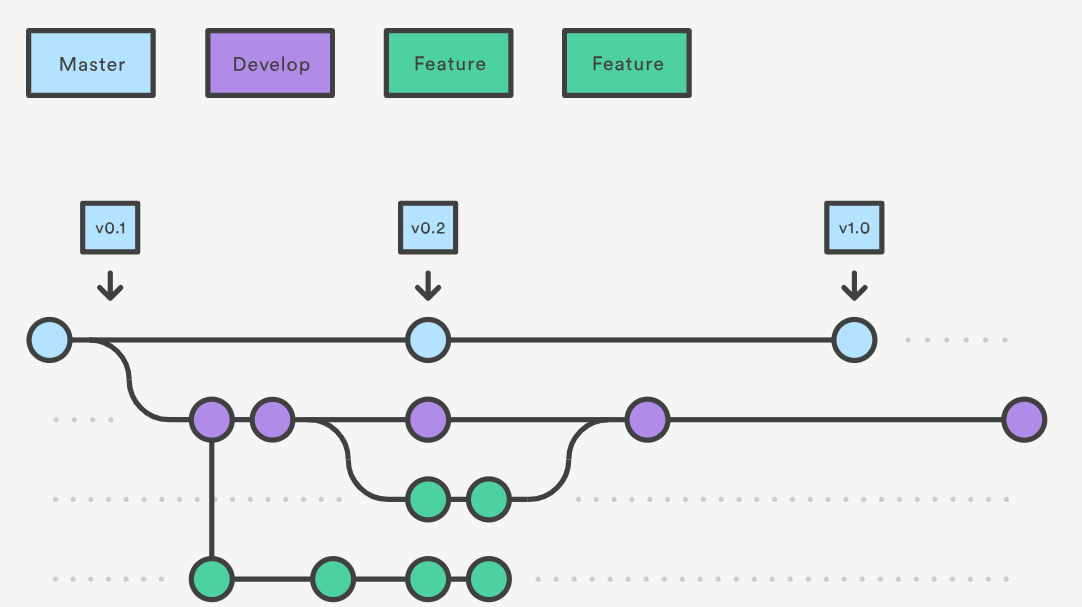
\includegraphics[width=0.7\textwidth]{img/gitbranches.PNG} % requires the graphicx package
  \caption{Git Workflow: Two stage release with feature-branch}
  \label{fig:gitworkflow}
\end{figure}
\subsection{Setup}
The steps below outline how to contribute source code to the project repository 
\begin{itemize}

\item Clone the Project
\begin{verbatim}
git clone https://gitlab.cas.mcmaster.ca/velechva/capstone.git
\end{verbatim}

\item Add a Feature Branch
\begin{verbatim}
git pull
git checkout develop
git checkout -b BRANCH_NAME
\end{verbatim}

\item Push Changes to Repository
\begin{verbatim}
git add FILE_NAME
git commit -m "MESSAGE"
git push 
\end{verbatim}



\end{itemize}

\subsection{Versioning Scheme}
The version number for the system will be updated every time a feature is revised or added. The scheme for versioning will follow the \textit{major.minor.patch} convention. The major number will increment by one when a new feature is introduced, or specifications for an existing feature are changed  The minor number will also increment by one, however only when features are refined. Fixing bugs will change the \texit{patch} number, incrementing it by one. 


\section{Process Workflow}

The development of systems will be spread out over the upcoming two months with three hour sessions every Friday. Work that is not completed will either cause the current session time to be extended, or be pushed to the next session. The team will also meet regularly on Thursdays to plan any work required for upcoming deadlines, and schedule them accordingly. These meetings will also allow group members to adjust priorities before the work is started. The goal will be to complete any outstanding deliverables three days before the actual deadline. The reason behind setting the deadline earlier then the actual due date is so that the team can review the work that has been completed. Task tracking will also be apart of the process work flow and will be done through software such as JIRA, Redmine, or Trello. The task tracking will inform team members on the status of tasks and what each individual member is working on. 

Hardware design and construction will follow the rapid application development process similar to Figure \ref{fig:rapid}. The ability to build multiple iterations quickly will help improve the design and allows the software to be tested instantly. Portions of the hardware systems will be built incrementally as well and integrated once they prove to be stable and efficient. The hardware will also be designed using off the shelf components to allow faster iterations. Using agile methodology and rapid application development allows the team to make multiple iterations which is beneficial since the TAs and/or Dr. Alan Wassyng will be able to give feedback quickly and allow the team to refine the prototype. 




\begin{figure}
	\centering
	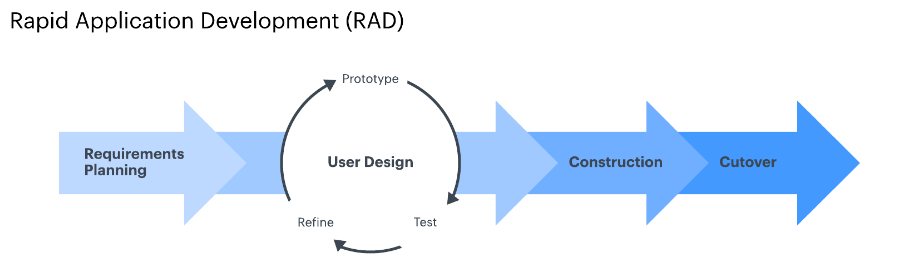
\includegraphics[width=.8\textwidth]{img/rad.png}
	\caption[]{Rapid Prototyping Development Processes}
	\label{fig:rapid}
\end{figure}


\end{document}  